\section{Benchmark Accuracy
of Victim and Surrogate Models}
\label{app:bench}

We report zero-shot accuracy of R1, \texttt{R1-Distill} (R1-Weak), and GPT-5.4-mini on MATH500, JEEBench, and LiveCodeBench (\textbf{LCB}) in Table~\ref{tab:benchmark_results}.

%--table 6
\begin{table}[h]
  \centering
  \caption{\textbf{Benchmark accuracy (\%) of victims and surrogates.} }
  \label{tab:benchmark_results}
  \small
  \setlength{\tabcolsep}{8.5pt}
  \begin{tabular}{lccc}
    \toprule
    \textbf{Model} & \textbf{MATH500} & \textbf{JEEBench} & \textbf{LCB} \\
    \midrule
    R1          & 91.6 & 87.1 & 74.9 \\
    R1-Distill  & 81.4 & 32.6 & 27.6 \\
    GPT-5.4-mini  & 91.4 & 85.1 & 66.9 \\
    \bottomrule
  \end{tabular}
  \vskip -0.1in
\end{table}


\section{Prompts for Compression and Zero-shot Trace Inversion}

\phantomsection
\label{box:summarization_prompt}
\begin{tcolorbox}[breakable, pad at break*=1mm, title=Reasoning Summary Compression Prompt]

\textbf{System prompt.}\\
You are summarizing a long chain-of-thought trace into a short, first-person ``inner-monologue recap'' that mirrors the style of GPT-5 mini's internal reasoning summaries.\\

Given a \texttt{<think>...</think>} trace, produce a recap with these properties:\\

\textbf{Structure.} Write 3 to 6 short sections. Each section begins with a short bold markdown header on its own line, like \texttt{**Setting up the integral**} or \texttt{**Checking the edge case**}, and is followed by one short paragraph (2--5 sentences). Do NOT use numbered lists (\texttt{1.}, \texttt{2.}) and do NOT use bullet points (\texttt{-}, \texttt{*}). The whole recap is just headers + prose.\\

\textbf{Voice.} First person, present tense, as if the model is thinking aloud: ``I need to\ldots'', ``I'll check\ldots'', ``I'm now realizing\ldots'', ``Let me verify\ldots''. Keep the tone tentative and exploratory, not textbook.\\

\textbf{Content.} Each section should capture one meaningful move in the reasoning --- a clarification of what is being asked, a key derivation or substitution, a pivot after a failed attempt, a sanity check, or the final consolidation. Skip filler, restatement, and purely mechanical arithmetic. Preserve the logical order of the trace.\\

\textbf{Length.} Aim for roughly 600--900 tokens total --- long enough that each section develops a real idea, not just a one-line gesture. If the input trace is very short, produce fewer sections rather than padding; if it is very long, prefer adding depth to each section over adding more sections.\\

\textbf{Math formatting.} Use inline LaTeX (\texttt{\textbackslash frac}, \texttt{\textbackslash sqrt}, \texttt{\textbackslash boxed}, etc.) where the original trace used math. Do not restate the final boxed answer unless the reasoning naturally concludes with it.\\

Do not add meta-commentary about following instructions, apologize, or mention that you are summarizing. Just produce the recap.\\

\vspace{-10pt}
\rule{\linewidth}{0.3pt}\\
\vspace{-10pt}

The prompt additionally includes two few-shot exemplars of the target style (one algebra / number theory and one geometry, $\approx$600 tokens each), drawn from GPT-5-mini's own summaries. They are omitted from this box for space; the full prompt including exemplars is released with our code.\\

\vspace{-10pt}
\rule{\linewidth}{0.3pt}\\
\vspace{-10pt}

\textbf{User prompt.}\\
Summarize this thinking process as a first-person inner-monologue recap:\\
\texttt{<think>\{thinking\_content\}</think>}

\end{tcolorbox}


\phantomsection
\label{box:zero_shot_inversion_summary}
\begin{tcolorbox}[breakable, pad at break*=1mm, title=Zero-shot Inversion Prompt (With Summaries)]
You are a language model that reconstructs full internal reasoning traces from high-level bubble summaries.\\

You will be given:\\
- A problem **input** (e.g., a math or logic problem)\\
- A final **output** or solution\\
- A list of numbered **reasoning bubbles**, where each bubble summarizes one key insight, step, or decision made during the problem-solving process\\

These bubbles are **condensed summaries** of what was originally a much longer, richer internal thought process.\\
Your task is to reconstruct that full process.\\

Below are high-level bubble summaries representing condensed thoughts or decisions. Your task is to reconstruct the full thinking trace that might have led to each summary. For each bubble, expand it into a **detailed internal monologue or reasoning chain**, showing how one idea leads to the next.\\

Include:\\
- Assumptions and background intuitions\\
- Intermediate steps, definitions, and subcases\\
- Natural questions or doubts raised during reasoning\\
- Alternatives that were considered and rejected\\
- Transitions that make the reasoning coherent and plausible\\

Use informal, introspective language — as if the person is thinking out loud. Add math expressions in \LaTeX where appropriate.\\

Do **not** invent new reasoning steps outside the bubbles. Use the **input** and **output** only for context and consistency. Your goal is to **flesh out the bubbles**, not to re-solve the problem from scratch.\\

The full trace should:\\
- Be logically consistent and cohesive from start to finish\\
- Sound like a realistic thought process that could plausibly result in the given answer\\
- Span multiple paragraphs per bubble and up to 20,000 characters overall if needed\\
- Be output as one continuous trace, wrapped in `<think>...</think>` tags\\

You are not summarizing the bubbles. You are recovering the internal narrative that *generated* them.\\

The original problem input is: \texttt{\{user\_prompt\}}\\
The final answer is: \texttt{\{assistant\_answer\}}\\
Transform this thinking bubbles into clear full reasoning traces: \texttt{\{reasoning\_summary\}}\\
\textbf{Generate full reasoning traces:}

\end{tcolorbox}


\newpage
\phantomsection
\label{box:zero_shot_inversion_no_summary}
\begin{tcolorbox}[breakable, pad at break*=1mm, title=Zero-shot Inversion Prompt (No Summaries)] 
You are a language model that reconstructs full internal reasoning traces from only an **input** (e.g., a math or logic problem) and a corresponding **output** (final solution or answer). \\

You will be given:\\
- A problem **input**\\
- A final **output** or solution\\

Your task is to reconstruct the full internal reasoning process that could plausibly connect the input to the output. This should be a long, detailed, introspective trace, not a short summary.\\

Guidelines for the reasoning trace:\\
- Write in the style of an informal, introspective monologue, as if the person is thinking out loud.\\
- Include assumptions, intuitions, and background facts as they arise naturally.\\
- Show intermediate steps, calculations, logical deductions, definitions, and subcases.\\
- Raise natural questions or doubts during reasoning, and explain how they are resolved.\\
- Explore alternative approaches, even ones that are discarded, and explain why.\\
- Make transitions clear so the reasoning feels like a coherent train of thought.\\
- Use \LaTeX for math expressions where helpful.\\
- Do not introduce new information inconsistent with the input or output.\\
- The goal is depth, not brevity: expand ideas fully, elaborate with multiple paragraphs, and let the reasoning unfold gradually.\\
- The output should only appear at the end, after the reasoning is complete.\\

The full trace should:\\
- Wrapped in <think>...</think> tags.\\
- Be logically consistent and cohesive from start to finish.\\
- Sound like a realistic thought process that could plausibly result in the given answer.\\
- Span thousands of tokens if needed.\\

The original problem input is: \texttt{\{user\_prompt\}}\\
The final answer is: \texttt{\{assistant\_answer\}}\\
\textbf{Generate full reasoning traces:}
\end{tcolorbox}


\newpage
\section{Examples of Synthesized Reasoning Traces}

%figure 4
\begin{figure*}[!ht]  
  \centering    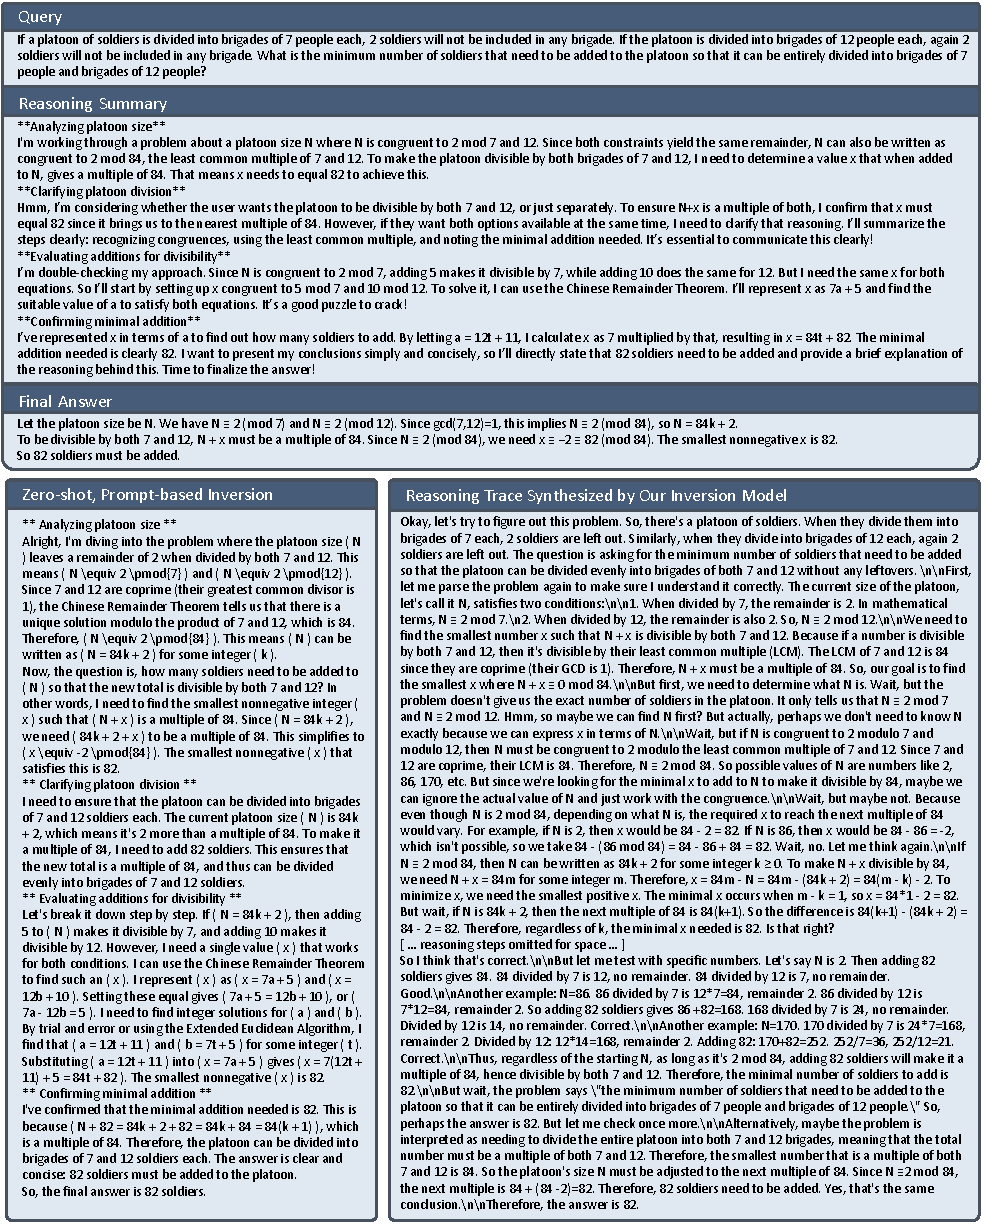
\includegraphics[width=\linewidth]{images/example_2.pdf}
  \caption{\textbf{Trace inversion against R1.} Zero-shot inversion versus trace inversion with \textbf{R1-Distill} as the surrogate model.}
  \vskip -0.2in
  \label{fig:example_2}
\end{figure*}

%figure 5
\begin{figure*}[!ht]
  %\vskip 0.1in
  \centering    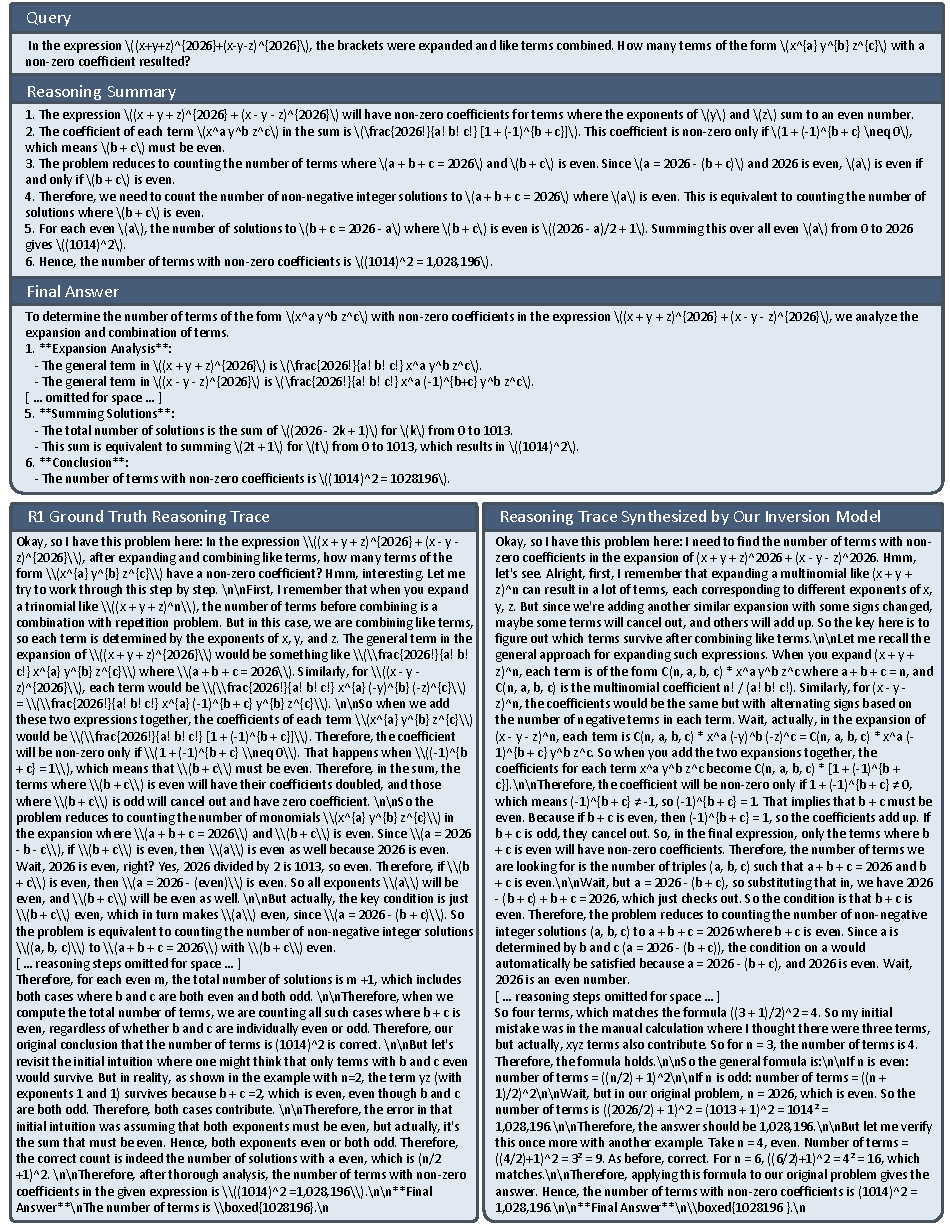
\includegraphics[width=\linewidth]{images/example_3.pdf}
  \caption{\textbf{Trace inversion against R1.} Ground-truth reasoning trace versus a trace synthesized with \texttt{R1-Distill} as the surrogate model.}
  \label{fig:example_3}
\end{figure*}


%\newpage
\clearpage
\section{Synthesized Traces Can Be Better Than Ground-Truth Traces}
\definecolor{qbg}{HTML}{E0E9F1}
\definecolor{qframe}{HTML}{475B78}
\definecolor{invbg}{HTML}{E0E9F1}
\definecolor{invframe}{HTML}{475B78}
\definecolor{r1bg}{HTML}{E0E9F1}
\definecolor{r1frame}{HTML}{475B78}
\definecolor{boxbrand}{HTML}{475B78}
\definecolor{hlbrand}{HTML}{C62828}

%figure 6
\begin{figure*}[h]
  \centering

\begin{tcolorbox}[
    colback=qbg, colframe=qframe,
    title={\small\textbf{Query}},
    fonttitle=\sffamily, fontupper=\small,
    boxrule=0.6pt, arc=2pt, left=4pt, right=4pt, top=2pt, bottom=2pt,
  ]
  The positive reals $x$ and $y$ satisfy $x^3 + y^3 = x - y$. Show that $x^2 + y^2 < 1$.
\end{tcolorbox}

\begin{minipage}[t]{0.485\textwidth}
  \begin{tcolorbox}[
    colback=r1bg, colframe=r1frame,
    title={\small\textbf{R1 Ground-Truth Reasoning Trace}},
    fonttitle=\sffamily, fontupper=\footnotesize,
    boxrule=0.6pt, arc=2pt, left=4pt, right=4pt, top=2pt, bottom=2pt,
  ]
  \ldots{} \textcolor{hlbrand}{\textit{Wait, but we already have $x - y = (x + y)(S - P)$ from the equation above.}} Wait, let's step back.\ldots

  Since $f$ is convex for $a > 0$, by Jensen's inequality: $(x^3 + y^3)/2 \geq ((x + y)/2)^3$. \textcolor{hlbrand}{\textit{But not sure if helpful here.}}\ldots

  Since $x > y$, we can write $x = y + k$ where $k > 0$. Substitute into the equation: $(y+k)^3 + y^3 = k$. Expanding: $2y^3 + 3y^2 k + 3yk^2 + k^3 = k$. \textcolor{hlbrand}{\textit{But this seems complicated. Maybe not the best approach.}}\ldots

  The inequality becomes $xy < 2y/(x+y)$. Since $y > 0$, we can divide both sides by $y$: $x < 2/(x+y)$. Multiply both sides by $(x+y)$: $x(x + y) < 2$. So $x^2 + xy < 2$. \textcolor{hlbrand}{\textit{But we need to relate this to our previous expressions. Hmm, not sure if helpful.}}\ldots
  \end{tcolorbox}
\end{minipage}
\hfill
\begin{minipage}[t]{0.485\textwidth}
  \begin{tcolorbox}[
    colback=invbg, colframe=invframe,
    title={\small\textbf{Synthesized Reasoning Trace}},
    fonttitle=\sffamily, fontupper=\footnotesize,
    boxrule=0.6pt, arc=2pt, left=4pt, right=4pt, top=2pt, bottom=2pt,
  ]
  Another idea: \ldots\ $x^2 - xy + y^2 = (x-y)/(x+y)$. But $x^2 + y^2 = (x^2 - xy + y^2) + xy$, so $x^2 + y^2 = (x-y)/(x+y) + xy$.

  Let's denote $t = y/x$, since $x > y$, so $t$ is a positive real number less than 1. \ldots\ substitute into the equation $x^3 + y^3 = x - y$: $x^3(1 + t^3) = x(1 - t)$. Therefore, $x^2 = (1 - t)/(1 + t^3)$. Now, $x^2 + y^2 = x^2(1 + t^2) = (1 - t)(1 + t^2)/(1 + t^3)$.

  \ldots\ Expand the left-hand side: $1 + t^2 - t - t^3 < 1 + t^3$. \ldots\ Factor out a $t$: $t(2t^2 - t + 1) > 0$. Discriminant $D = (-1)^2 - 4 \times 2 \times 1 = 1 - 8 = -7$. Since the discriminant is negative, the quadratic $2t^2 - t + 1$ has no real roots and since the coefficient of $t^2$ is positive, it is always positive. \ldots\ we conclude that $x^2 + y^2 < 1$.''\ldots
  \end{tcolorbox}
\end{minipage}
  \caption{\textbf{R1 ground-truth trace vs.\ synthesized trace with R1 as the surrogate.} \textbf{Top:} the query. \textbf{Bottom left:} excerpt from R1's ground-truth trace, which tries and abandons several approaches.
  %(\textcolor{hlbrand}{highlighted}). 
  \textbf{Bottom right:} matching excerpt from the trace synthesized by our inversion model (trained with R1 as the surrogate), with more direct reasoning.}
  \label{fig:r1_vs_inverter_backtrack}
\end{figure*}
